\chapter{Ewaluacja}

\subsection{Odometria}
\label{sec:odometry}
Robot korzysta z nawigacji zliczeniowej w celu połączenia pomiarów odległości zebranych z otoczenia i aproksymacji ich położenia na płaszczyźnie względem jednego ustalonego punktu. Zliczaniu podlegają dwie wartości - dystans przejechany wzdłuż oraz obrót pojazdu w miejscu. Szereg zmierzonych w ten sposób wartości umożliwia odtworzenie przejechanej ścieżki. Rys. \ref{fig:odom-axis-simplified} przedstawia rzeczywisty oraz uproszczony model podwozia robota. Zamiast uwzględniać obie poziome osi i 4 koła, upraszcza się go do formy robota o jednej osi, z jedną parą kół. Gdy oba koła poruszają się w tę samą stronę, robot przesuwa się w przód lub w tył. Gdy pracują przeciwbieżnie - obraca się wokół punktu oznaczonego znakiem X.

\begin{figure}[H]
	\centering
		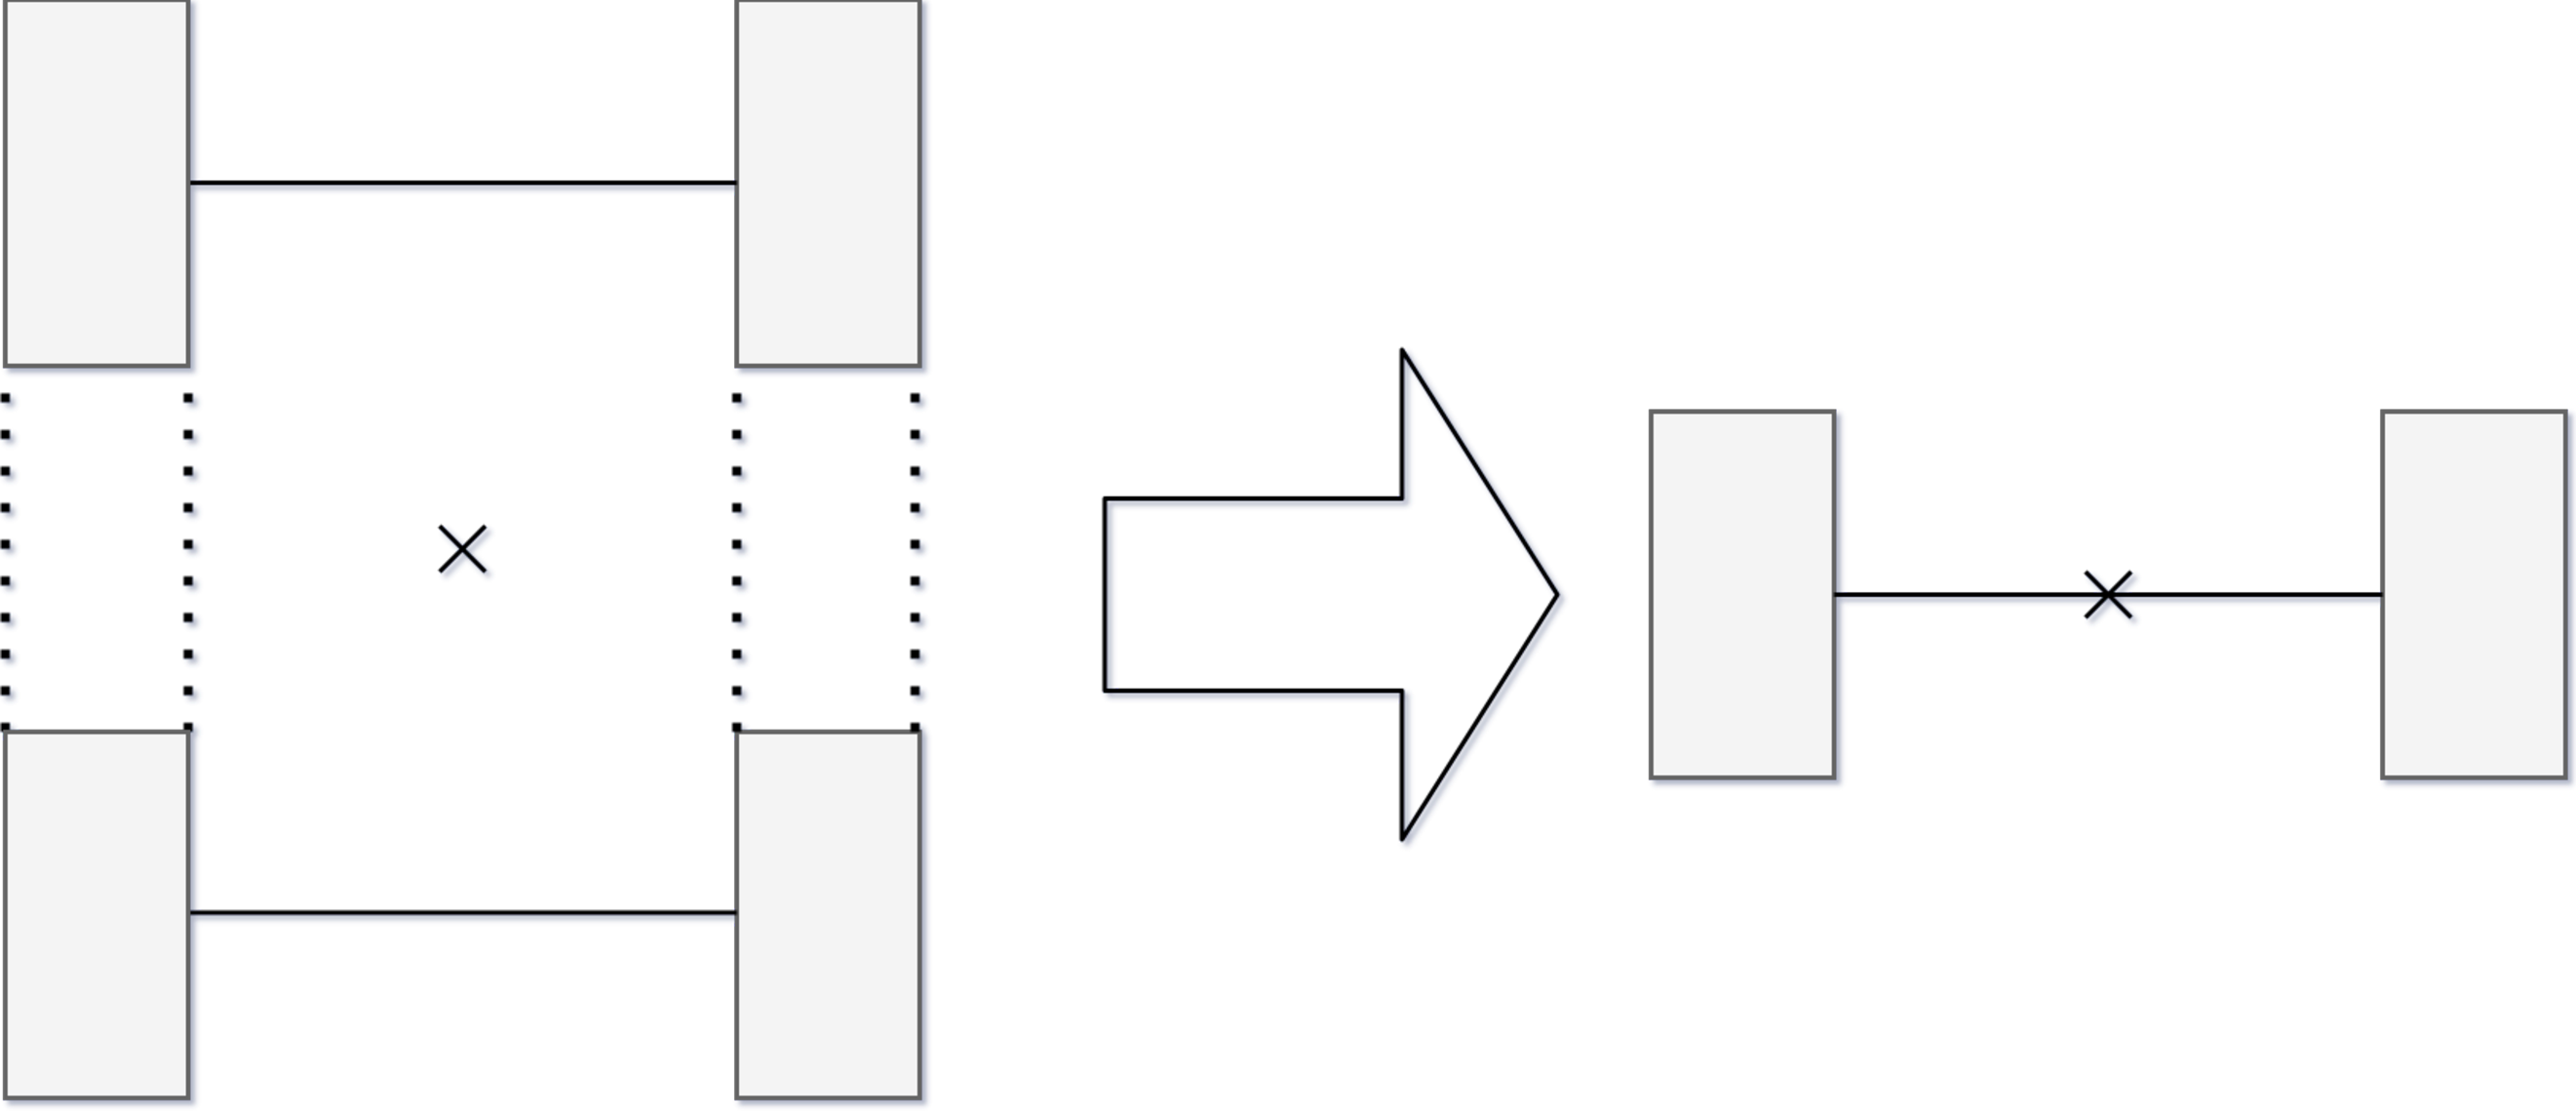
\includegraphics[width=0.6\linewidth]{rys/robot-odometry-simplified.pdf}
	\caption{Model rzeczywisty i uproszczony (X oznacza środek robota - pionową oś wokół której się obraca)}
	\label{fig:odom-axis-simplified}
\end{figure}


Pierwszym pomysłem było wykorzystanie enkoderów do pomiaru translacji pojazdu wzdłuż jego osi ruchu, pozostawiając zliczanie obrotu funkcjom korzystającym z magnetometru.

\begin{figure}[H]
	\centering
		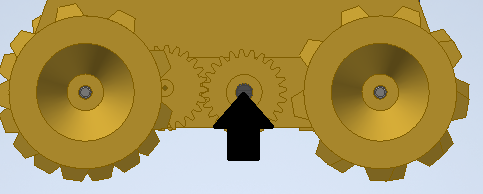
\includegraphics[width=0.5\linewidth]{rys/encoder-position.png}
	\caption{Umiejscowienie enkodera z prawej strony robota}
	\label{fig:encoder-pos}
\end{figure}

Enkodery zostały zamontowane w miejscu przedstawionym na Rys. \ref{fig:encoder-pos}, symetrycznie po obu stronach podwozia. Napęd podany od serwa przez zębatkę przenosi napęd zarówno na tylne koło jak i enkoder, z przekładniami 1:1 w obu przypadkach. Dzięki takiemu rozwiązaniu pełny obrót enkodera odpowiada pełnemu obrotowi koła. Enkoder obrotowy EC-11 generuje 20 impulsów przy kącie obrotu 360°. Aby można było wyznaczyć pokonaną odległość, w pierwszej kolejnosci należy obliczyć stosunek ilości impulsów do przejechanego dystansu - w tym celu autor stworzył prosty wzór:

\begin{center}
    $DPR = \frac{2 \pi r}{p}$ \\
    \emph{DPR - współczynnik (ang. Distance to Pulse Ratio) wyrażany w cm/impuls} \\
    \emph{r - promień koła pojazdu} \\
    \emph{p - liczba impulsów enkodera na obrót koła}
\end{center}

Wiedząc ile impulsów generuje enkoder, oraz znając wymiary koła w łatwy sposób można obliczyć DPR. Podstawiając dane to jest:

\begin{center}
    $DPR = \frac{2 \pi 2,5cm}{20imp}$ \\
    $DPR = 0.785 \frac{cm}{imp}$ \\
    $\frac{1}{DPR} = 1.274$
\end{center}

Znając współczynnik aby obliczyć przejechany dystans wystarczy zmierzyć ilość impulsów jakie wystąpiły podczas przejazdu a następnie pomnmożyć je przez DPR. Otrzymany wynik oznacza przesunięcie robota wyrażone w centymetrach. Jako że platforma posiada dwa enkodery, a nie jest możliwe zachowanie idealnie prostego toru jazdy, wyciągana jest średnia liczba impulsów. Ze względu na grubość i wypustki na gąsienicach oraz ich poślizg rzeczywisty dystans przejechany będzie inny od zadanego. Dla kompensacji tej różnicy wartość DPR została skorygowana ręcznie do takiej, przy której błąd przemieszczenia robota zawierał się w granicy ±10\% na zadanym dystansie 100cm. Widoczna w kodzie programu, skorygowana wartość $\frac{1}{DPR}$ wynosi $1.325$ co odpowiada $DPR=0.755$ . Poniższy listing prezentuje funkcję realizującą to zadanie.


\begin{lstlisting}[basicstyle=\footnotesize\ttfamily,language=c++,caption=Fragment kodu obsługującego polecenie \emph{MOVE},label=lst:move]
//MOVE
case 9:
{
    reset_encoders();
    float val = getArgument(command, 1).toInt() * 1.325;

    if (val > 0)
        driveMotors(90, 90);
    else
        driveMotors(-90, -90);

    val = abs(val);
    while ((left_encoder_counter + right_encoder_counter) / 2 < val)
    {
    }

    driveMotors(0, 0);
    delay(100);
    Serial2.println("OK");
}
\end{lstlisting}

Podczas wykonywania polecenia \emph{MOVE} na gąsienice zadawana jest pełna prędkość i w pętli sprawdzana jest średnia ilość impulsów wygenerowanych przez enkoder. Dla optymalizacji algorytmu, zamiast przeliczać przy każdym pomiarze ilość impulsów razy wartość DPR, na początku zadana w parametrze wartość odległości jest mnożona przez $\frac{1}{DPR}$, i dalej w takiej formie ta wartość wykorzystywana przy operacji porównania. W momencie w którym średnia zliczona ilość impulsów przekroczy jej wartość, serwa zostają zatrzymane.
\\ 

Obrót (funkcja \emph{ROTATE}) polega na zadaniu przeciwstawnych wartości prędkości na obie gąsienice. W celu obrotu poruszają się one przeciwbieżnie, z równymi prędkościami. Pierwsza implementacja funkcji obrotu wyglądała jak przedstawiono poniżej:

\begin{lstlisting}[basicstyle=\footnotesize\ttfamily,language=c++,caption=Funkcja będąca głównym elementem obsługi poleceń \emph{ROTATE} oraz \emph{ROTATE\_TO},label=lst:rotate-to-function]
void rotateTo(int azimuth)
{
    if (calcAngleDistance(getAzimuth(), azimuth) > 0)
        driveMotors(-90, 90);
    else
        driveMotors(90, -90);

    while (true)
    {
        if (abs(calcAngleDistance(getAzimuth(), azimuth)) <= 10)
            break;
        delay(10);
    }
    driveMotors(0, 0);
    delay(100);
}
\end{lstlisting}

Na początku mierzony jest azymut początkowy i obliczany jest azymut końcowy (tj. początkowy + zadana wartość obrotu). Dalej wykonywana jest ta sama funkcja co w przypadku \emph{ROTATE\_TO} przyjmująca parametr azymutu końcowego. Podczas obrotu, w pętli, sprawdzana jest różnica kąta aktualnego od zadanego. Jeżeli wartość bezwzględna obrotu znajdzie się w zakresie ±10° robot zatrzyma się.

Takie rozwiązanie jest dobre, o ile magnetometr jest skalibrowany i funkcjonuje poprawnie. Niestety, podczas skanów okazało się że nie można polegać na pomiarach z tego sensora - więcej o tym znajduje się w sekcji \ref{sec:scan}. Z tego powodu koniecznym okazała się zmiana podejścia do pomiaru obrotu.

Poniższy listing przedstawia nowe podejście osbługi polecenia \emph{ROTATE}. Jest ono mniej dokładne od poprzedniego, bardziej podatne na dryf (błąd obrotu kumuluje się), natomiast taki pomiar jest odporny na zakłócenia pola magnetycznego.
Tym razem procedura jest analogiczna jak w przypadku ewaluacji polecenia \emph{MOVE}. W pętli sprawdzana jest średnia ilość impulsów, jednak tym razem gąsienice poruszają się przeciwbieżnie. Kąt obrotu na początku należy przemnożyć przez pewien współczynnik tak aby odpowiadał on ilości impulsów. Platforma kończy ruch w momencie gdy średnia wartość przekroczy obliczony próg impulsów.

\begin{lstlisting}[basicstyle=\footnotesize\ttfamily,language=c++,caption=Nowa implementacja obsługi polecenia \emph{ROTATE},label=lst:rotate]
// ROTATE
    case 11:
    {
        reset_encoders();
        float val = getArgument(command, 1).toInt() * 0.164;
        if (val > 0)
            driveMotors(-90, 90);
        else
            driveMotors(90, -90);

        val = abs(val);
        while ((left_encoder_counter + right_encoder_counter) / 2 < val)
        {
        }

        delay(100);
        driveMotors(0, 0);
        Serial2.println("OK");
    }
    break;
\end{lstlisting}

Stosunek kąta obrotu do liczby impulsów ($0.164$) został wyznaczony eksperymentalnie. Najpierw przyjęto wartość 1. Następnie zadawany był kąt obrotu 90°, po czym mierzony był rzeczywisty kąt obrotu. Jeżeli wynosił on więcej, współczynnik redukowano o 0,1; analogicznie gdy obrót był mniejszy niż zadano. Gdy tak zgrubna regulacja była niewystarczająca (albo za mały albo za duży obrót), krok został zmniejszony do 0,05. Po kolejnej zmianie kroku do 0,02 czynność powtarzano do momentu w którym dalsza korekcja nie była konieczna. \\

Taka implementacja została zachowana do końca projektu. Polecenie \emph{ROTATE\_TO} dalej korzysta ze starego sposobu z użyciem magnetometru, jednak nie jest ono wykorzystywane podczas pomiarów.

\subsubsection{Kalibracja magnetometru}
%>TODOwspomnij o potrzebie zastosowania filtru (np kalmana)

Wykorzystywany w projekcie moduł magnetometru jest urządzeniem czułym i bardzo podatnym na zakłócenia - szczególnie jeśli mierzone jest pole magnetyczne ziemi. Poza zakłóceniami z otoczenia, występują również te wynikające z samej budowy robota - wszelkie przewody przez które płynie prąd generują swoje własne pola, nawet same metalowe elementy interferują z pomiarem. >TODO przypis o zakloceniach i ich zrodlach Na te zakłócenia należy zwrócić uwagę i podjąć kroki mające na celu ich kompensację. Warto też wspomnieć, że w tej pracy jednostki uzyskane z pomiaru nie mają znaczenia - jedyne co jest potrzebne w celu uzyskania informacji o kierunku w którym robot jest zwrócony to kierunek i zwrot zmierzonego wektora wartości natężenia pola.

Pierwszym problemem są zakłócenia typu \emph{hard iron}. Ich obecność przejawia się w postaci stałego przesunięcia mierzonych we wszystkich trzech osiach wartości natężenia pola magnetycznego. Zmierzone wartości można przedstawić na trójwymiarowym wykresie (jak uczyniono w pierwszych wersjach aplikacji sterującej). Każda z osi wykresu odpowiada osi pomiaru natężenia pola magnetycznego. W idealnej sytuacji zbór punktów powinien być osadzony na sferze o środku w punkcie $(0,0,0)$. Tak się jednak nie dzieje, co jest widoczne na Rys. \ref{fig:3d-mag-no-cal}.

\begin{figure}[ht]
	\centering
		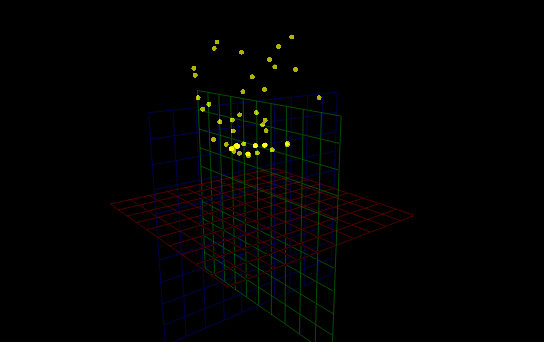
\includegraphics[width=0.6\linewidth]{rys/ScanBot-03-magnetometer-3d-decalibrated.PNG}
	\caption{Wykres obrazujący dane pozyskane z nieskalibrowanego magnetometru}
	\label{fig:3d-mag-no-cal}
\end{figure}

Aby dokonać korekcji \emph{hard iron} \cite{hard-iron}\cite{hard-soft-iron} dla każdej osi z osobna należy wyznaczyć minimalną i maksymalną zmierzoną wartość. Sumę obu wartości dzieli się przez 2, a uzyskana liczba to przesunięcie (ang. \emph{offset}). Aplikacja korekcji polega na odjęciu tej liczby od zmierzonej wartości.
Tą procedurę dla trzech osi przedstawiają kolejno Rys. \ref{fig:3d-mag-hard-corr-x}, Rys. \ref{fig:3d-mag-hard-corr-y} i Rys. \ref{fig:3d-mag-hard-corr-z}.

\begin{figure}[H]
	\centering
		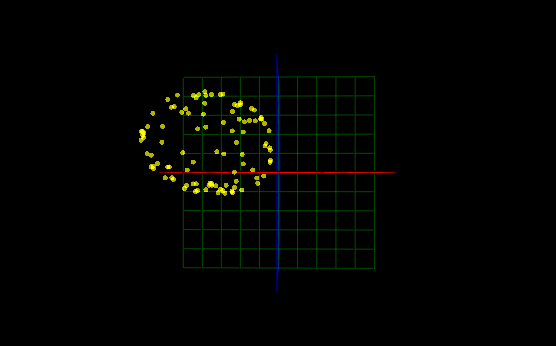
\includegraphics[width=0.6\linewidth]{rys/ScanBot-04-magnetometer-3d-calibration.PNG}
	\caption{Korekta przesunięcia \emph{hard iron} dla osi X}
	\label{fig:3d-mag-hard-corr-x}
\end{figure}

\begin{figure}[H]
	\centering
		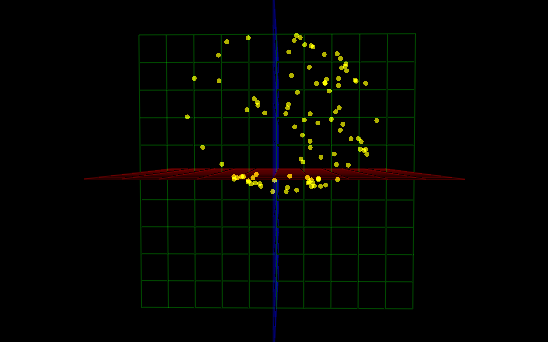
\includegraphics[width=0.6\linewidth]{rys/ScanBot-05-magnetometer-3d-calibration.PNG}
	\caption{Korekta przesunięcia \emph{hard iron} dla osi Y}
	\label{fig:3d-mag-hard-corr-y}
\end{figure}

\begin{figure}[H]
	\centering
		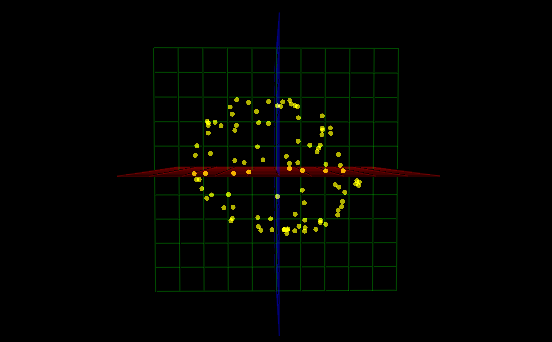
\includegraphics[width=0.6\linewidth]{rys/ScanBot-06-magnetometer-3d-calibration.PNG}
	\caption{Korekta przesunięcia \emph{hard iron} dla osi Z}
	\label{fig:3d-mag-hard-corr-z}
\end{figure}

Niestety, kształt chmury punktów wciąż daleki jest od idealnej sfery. Efektem tego jest nieliniowość uzyskanego azymutu - zmiana rzeczywistego kąta skierowania platformy względem zmiany zmierzonej będzie się znacząco różniła w zależności od początkowej pozycji. Ten efekt można by obejść za pomocą mapowania wartości przepuszczając odczyt przez funkcję odpowiedniej krzywej, jednak wymagałoby to formułowania skomplikowanego równania, bądź wyznaczenia arbitralnego przebiegu funkcji. Istnieje jednak mniej wymagające obliczeniowo podejście z zastosowaniem macierzy \cite{hard-soft-iron}. Dla uproszczenia obliczeń, zrezygnowano z pomiaru w trzech osiach, zamiast tego mierzone są jedynie natężenia pola w osiach X i Y (Rys. \ref{fig:2d-mag-no-cal}).

\begin{figure}[H]
	\centering
		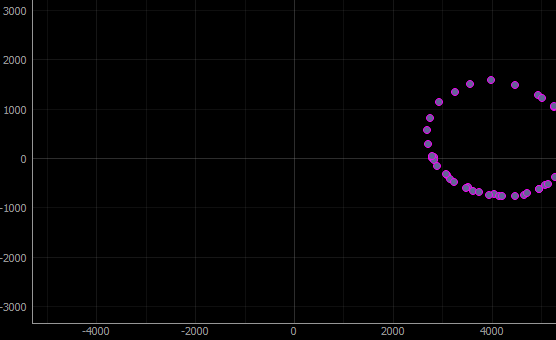
\includegraphics[width=0.8\linewidth]{rys/ScanBot-08-2d-calibration-theta-sigma.PNG}
	\caption{Rozkalibrowany magnetometr na dwuwymiarowej płaszczyźnie}
	\label{fig:2d-mag-no-cal}
\end{figure}

Tak jak w przypadku trzech wymiarów, w pierwszej kolejności dokonywana jest korekcja zniekształceń \emph{hard iron} na wszystkich osiach (Rys. \ref{fig:2d-mag-hard-corr-xy}).

\begin{figure}[H]
	\centering
		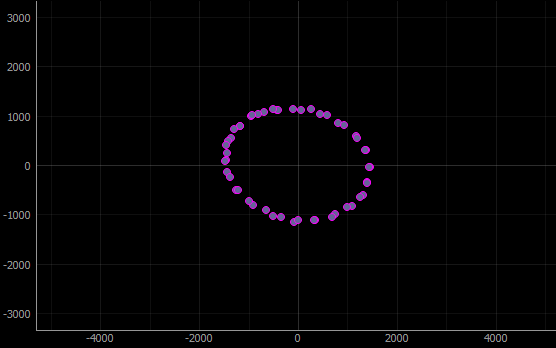
\includegraphics[width=0.8\linewidth]{rys/ScanBot-10-2d-calibration-theta-sigma-2-added-hard-offset-reset-data-so-soft-iron-values-are-proper.PNG}
	\caption{Korekcja hard iron}
	\label{fig:2d-mag-hard-corr-xy}
\end{figure}


Teraz można przystąpić do procedury kompensacji zniekształceń \emph{soft iron}. Idealnie, po dokonaniu korekcji w dwóch wymiarach, punkty na wykresie można by umieścić na okręgu - tak jednak nie jest. Uzyskany kształt bardziej przypomina elipsę, i ta właściwość zostanie wykorzystana. Proces przebiega w kilku krokach:

\begin{enumerate}
    \item Dla każdego z punktów liczony jest promień $r$ (wektor od $(0,0)$ do danego punktu)
    \item Wyznaczana jest maksymalna wartość promienia $rmin$ i $rmax$. Te wartości odpowiadają kolejno półosi małej i półosi wielkiej elipsy.
    \item Dla punktu odpowiadającego promieniowi $rmax$ Obliczany jest kąt $\theta$ za pomocą dwuargumentowej funkcji $arctan2(y,x)$, gdzie $x$ i $y$ są współrzędnymi punktu. Kąt ten odpowiada kątowi obrotu elipsy.
    \item Tworzona jest macierz $R$. Posłuży do obrotu elipsy.
    $R = \begin{bmatrix}
            cos\theta & sin\theta\\
            -sin\theta & cos\theta
        \end{bmatrix}$
    \item Obliczany jest parametr $\sigma$. Posłuży do ściskania elipsy. $\sigma = \frac{rmin}{rmax}$
    \item Za pomocą macierzy $R$ elipsa jest obracana o kąt -$\theta$ w celu zrównania jej wielkiej półosi z osią OX układu współrzędnych. Współrzędne każdego z punktów kolejno są osobno przekształcane za pomocą mnożenia macierzy:
    $   
        \mathit{v}_{2}
        =
        \begin{bmatrix}
            cos\theta & sin\theta\\
            -sin\theta & cos\theta
        \end{bmatrix}
        \times
        \begin{bmatrix}
            \mathit{v}_{1x}\\
            \mathit{v}_{1y}
        \end{bmatrix}
    $
    gdzie $\mathit{v}_{2}$ to wynikowy wektor zawierający współrzędne przekształconego punktu.
    \item Obróconą elipsę sprowadza się do postaci okręgu poprzez ściśnięcie jej w osi X. Robi się to przemnażając współrzędną x każdego z punktów osobno przez wcześniej obliczony parametr: $\mathit{v}_{2x} = \mathit{v}_{1x} \times \sigma$
\end{enumerate}

Ostatecznie chmura punktów tworzy okrąg co przedstawiono na Rys. \ref{fig:2d-mag-soft-corr-applied}. Efektem zastosowania kalibracji jest równomierny odczyt azymutu wraz z obrotem platformy. Każdy zmierzony i przefitrowany punkt może być teraz przeliczony na kąt wektora, który wskazuje azymut - wystarczy skorzystać z dwuargumentowej funkcji $arctan2(x,y)$, gdzie $x$ i $y$ są współrzędnymi punktu.

\begin{figure}[ht]
	\centering
		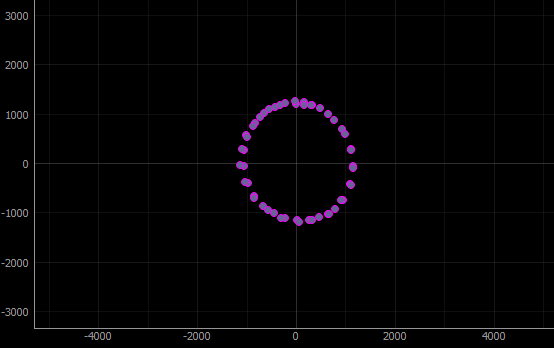
\includegraphics[width=0.8\linewidth]{rys/ScanBot-11-2d-set-theta-then-sigma-and-done.PNG}
	\caption{Chmura punktów po dokonaniu korekcji obu typów zniekształceń}
	\label{fig:2d-mag-soft-corr-applied}
\end{figure}

Finalna wersja aplikacji korzysta z dwóch osi magnetometru. W celu kalibracji należy skorzystać z zakładki \emph{magnetometer calibration} głównego okna aplikacji sterującej. Rys. \ref{fig:main-app-mag-section-bottom} przedstawia najważniejsze elementy tej zakładki, wykorzystywane podczas półautomatycznego procesu kalibracji.

\begin{figure}[ht]
	\centering
		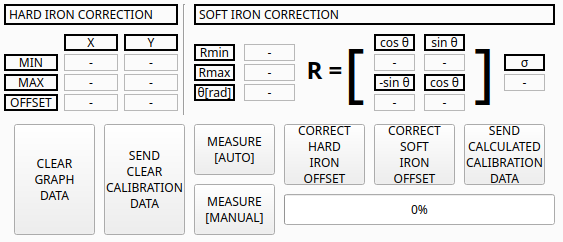
\includegraphics[width=1\linewidth]{rys/main-app-view-magnetom-bottom.png}
	\caption{Najważniejsze elementy sekcji kalibracji}
	\label{fig:main-app-mag-section-bottom}
\end{figure}

Aby dokonać kalibracji, robot powinien być połączony z aplikacją sterującą. Dalej procedura przebiega jak następuje:

\begin{enumerate}
    \item Należy przejśćdo zakładki \emph{magnetometer calibration}
    \item Jeżeli na wykresie znajdują się poprzednie pomiary, należy kliknąć przycisk \emph{CLEAR GRAPH DATA} aby je usunąć
    \item Należy wyzerować dane kalibracyjne znajdujące się w pamięci EEPROM robota. Służy do tego przycisk \emph{SEND CLEAR CALIBRATION DATA}
    \item Na tym etapie istnieją dwie możliwości przeprowadzenia pomiaru - za pomocą przycisku \emph{MEASURE [AUTO]} platforma samodzielnie, krokowo, wykona obrót wokół własnej osi i zbierze serię pomiarów z magnetometru; za pomocą przycisku \emph{MEASURE [MANUAL]} dokona jedynie pomiarów, w tym czasie należy robota obracać ręcznie. Postęp pomiarów wizualizowany jest na pasku postępu w prawym dolnym rogu. Na wykresie pojawią się zebrane pomiary. W sekcji oznaczonej \emph{HARD IRON CORRECTION} pojawiać się będą uzyskane dane dotyczące korekcji pierwszego z omawianych wcześniej zaburzeń - wartości minimalne i maksymalne dla każdej z osi oraz wartość przesunięcia (\emph{OFFSET}). W sekcji \emph{SOFT IRON CORRECTION} pojawiać się będą cyklicznie przeliczane wartości dotyczące korekcji zaburzeń \emph{soft iron} - m.in. parametry $\theta$ $\sigma$ i wartości macierzy $R$.
    \item Za pomocą przycisku \emph{CORRECT HARD IRON OFFSET} należy dokonać korekcji zaburzeń typu \emph{hard iron} na podstawie obliczonych wartości przesunięcia. Efekt natychmiastowo ukaże się na wykresie.
    \item Za pomocą przycisku \emph{CORRECT SOFT IRON OFFSET} należy dokonać korekcji zaburzeń typu \emph{soft iron}. Dane również brane są z obliczonych podczas procedury pomiaru. W tym momencie punkty na wykresie powinny być ułożone w okrąg. Jeżeli jest inaczej, oznacza to że w otoczeniu występują zaburzenia pola magnetycznego. Wtedy należy przemieścić robota w inne miejsce i powtórzyć wymienione czynności od nowa.
    \item Na koniec, aby wysłać dane kalibracyjne do robota, należy kliknąć przycisk \emph{SEND CALCULATED CALIBRATION DATA}. 
\end{enumerate}

Po dokonaniu procedury kalibracji pomiary dużo lepiej oddają rzeczywisty kierunek i zwrot platformy, jednak nawet podczas postoju platformy zwracana wartość azymutu nie pozostaje stała. Aby zniwelować to zjawisko konieczne jest zastosowanie filtru. W tego typu sensorach powszechnie wykorzystywany jest filtr Kalmana.

\subsubsection{Filtr Kalmana}






\subsection{Skan otoczenia i budowa mapy}
\label{sec:scan}
%>TODO powiedz o tym jak sie skaszaniło przy przewodzie pod podłogą<<<<<<<<<<<<<< koniecznie tutaj

Samo zebranie pomiarów i przedstawienie ich w formie czytelnej dla człowieka nie jest trudne w realizacji. Pozyskane dane można przedstawić na wykresie, punkty połączyć prostymi liniami. Problem zaczyna się z agregacją wielu pomiarów, i na tym będzie koncentrował się ten rozdział.

Mając do dyspozycji sensory


%>TODO tu napisac o bazowym mapowaniu pkt na plaszczyzne
%o swojej implementacji ze scorem
%nastepnie o tym co moznaby dalej (translacja korekta)
%ale nie zostalo zrobione bo bylo slabe i to wymaga filtrow czasteczek
%i ze jest cos takiego jak cartographer od googla
%ale zdecydowano ze gmapper jest spoko i czemu nie gmapper


%%przewod - interferencja
\begin{figure}[ht]
	\centering
		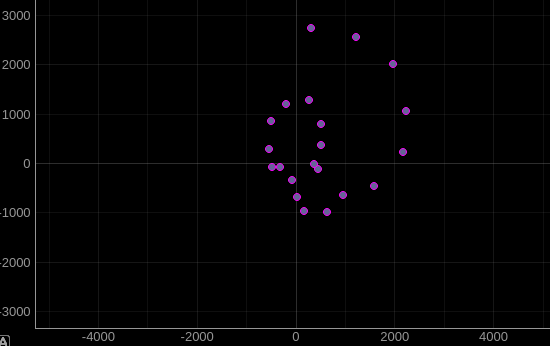
\includegraphics[width=0.8\linewidth]{rys/calibrated-mag-high-interference-broken-rotation.PNG}
	\caption{>TODO}
	\label{fig:xxx}
\end{figure}

%% znowu przewod
\begin{figure}[ht]
	\centering
		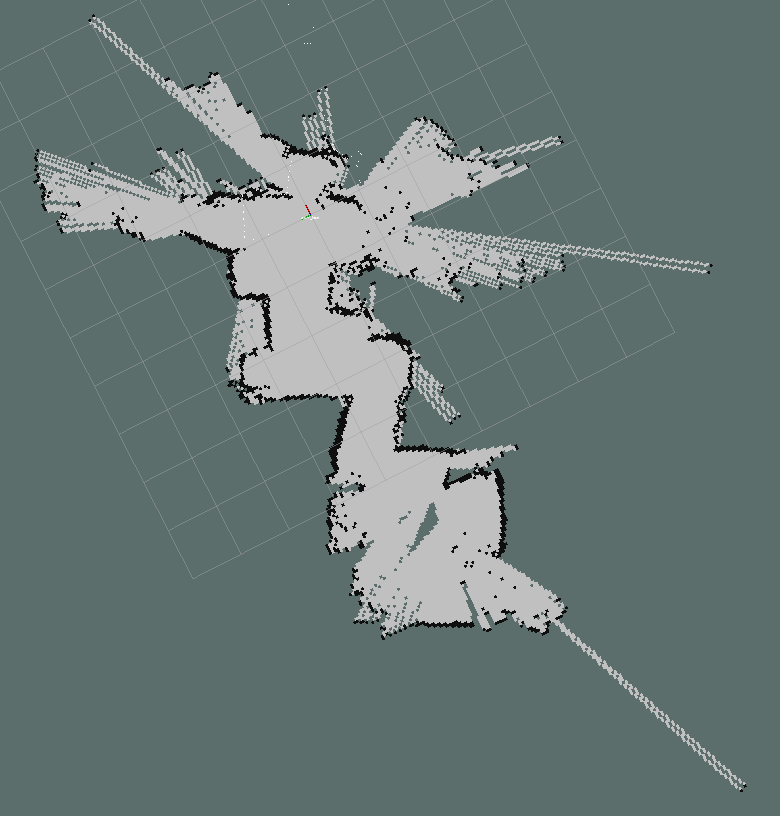
\includegraphics[width=0.8\linewidth]{rys/2020-11-04-170347_1920x1080_scrot.PNG}
	\caption{>TODO}
	\label{fig:xxx}
\end{figure}


\begin{figure}[ht]
	\centering
		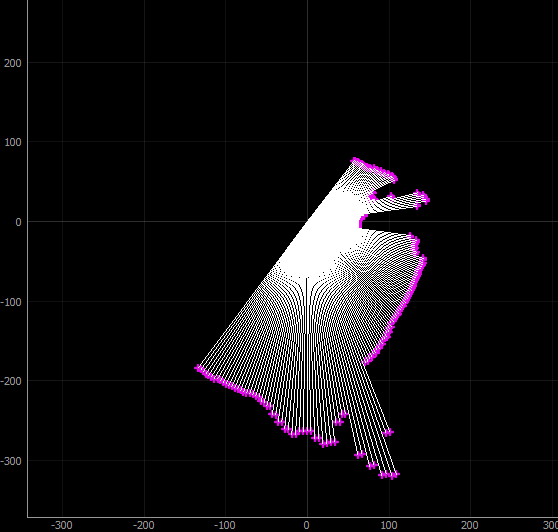
\includegraphics[width=0.5\linewidth]{rys/ScanBot-12-calibrated-room-map1.PNG}
	\caption{>TODO}
	\label{fig:xxx}
\end{figure}

\begin{figure}[ht]
	\centering
		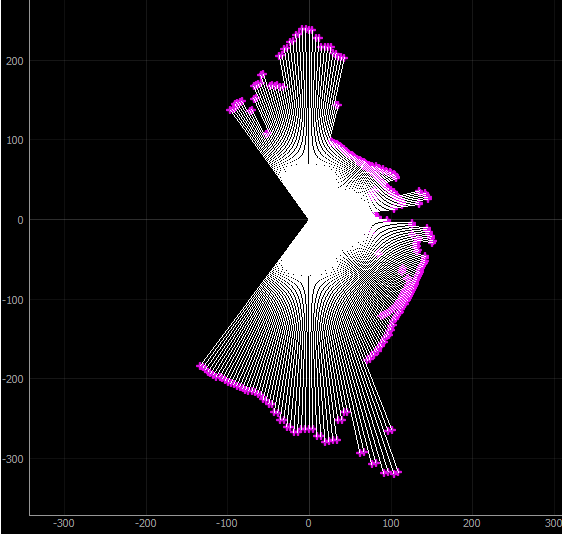
\includegraphics[width=0.5\linewidth]{rys/ScanBot-12-calibrated-room-map2.PNG}
	\caption{>TODO}
	\label{fig:xxx}
\end{figure}

\begin{figure}[ht]
	\centering
		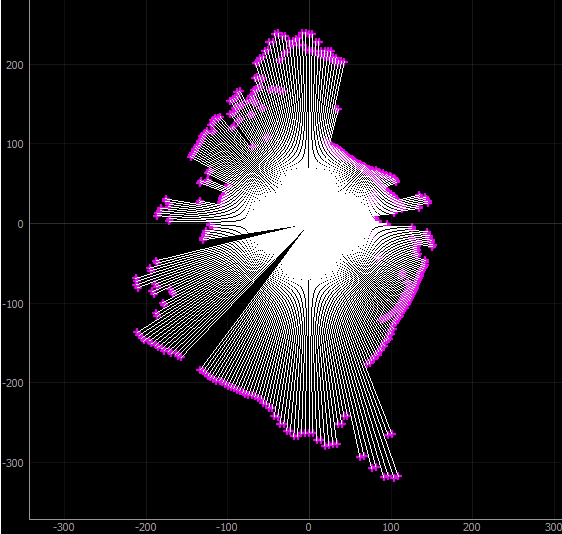
\includegraphics[width=0.5\linewidth]{rys/ScanBot-12-calibrated-room-map3.PNG}
	\caption{>TODO}
	\label{fig:xxx}
\end{figure}

\begin{figure}[ht]
	\centering
		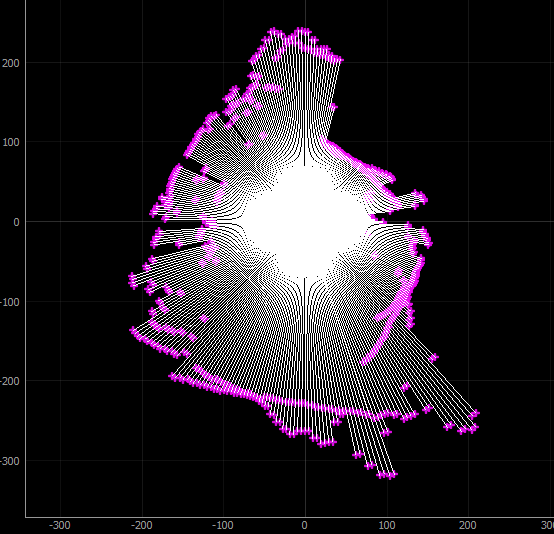
\includegraphics[width=0.5\linewidth]{rys/ScanBot-12-calibrated-room-map4.PNG}
	\caption{>TODO}
	\label{fig:xxx}
\end{figure}


\subsubsection{UMBenchmark\cite{Borenstein1995}}
%>TODO tu dac fotki koniecznie
%jakies rysunki nabazgrane z kwadratami
% i powiedziec ze sie nie pokrywalo najlepiej
% dac tabelke z pozycjami
% pokazac obliczenia center of gravity itd
% wyszlo ~1proc czyli to bez sensu
% wiec robot juz jezdzi wystarczajaco dobrze

% >TODO nawiaz do wczesniej wspomnianych rzeczy
% powiedz co po kolei jak sie zmieniało
% z czym były problemy
% o tutaj mala podpowiedz:

% sensor dzwieku jest do kitu za duza fluktuacja pluz ogromny kąt plus za duzy blad pomiaru plus za dlugi pomiar
% sharp mniejszy kąt mniejsza fluktuacja krotki pomiar ale podatnosc na swiatlo
% lidar super miodzio
% serwo kiepskie i wibruje/zacina się co powoduje błędy na krawędziach
% magnetometr-biblioteka koryguje jedynie hard iron i jest do kitu
% ze wzgledu na moc obliczeniowa najlepiej bylo samemu zaimplementowac soft i hard iron
% zeby bylo prosciej tylko 2 wymiary, niestety nie kompensujemy tiltu. ale i tak zalozenie jest ze jezdzimy po plaskim

% używanie arcsin zamiast atan2 z ifami podowowało błąd że correction czasem obracał elipsę nie w tę stronę